\section{Werde zum Tennisspieler}
In dieser Aufgabe bauen wir ein kleines Tennisspiel, das auch unter dem Namen  \emph{Pong} bekannt ist.Ziel des Spieles ist es einen Ball mit dem Schläger zu treffen. Verfehlt man den Schlag und trifft der Ball hinter einem auf den Rand, so erhält der Gegner einen Punkt. Wer als erster 10 Punkte erlangt hat, hat gewonnen.
\subsection{Programmiere einen Spieler}
Wir brauchen für das Spiel zwei Spieler. Beide verhalten sich gleich, daher reicht es einen Spieler zu malen und ihn im Anschluss zu kopieren. Wir erzeugen dazu ein weiteres Sprite.

\subsubsection{Male den Spieler}
\begin{enumerate}
\item Klicke auf das \textit{Neues Objekt malen}-Icon
\end{enumerate}
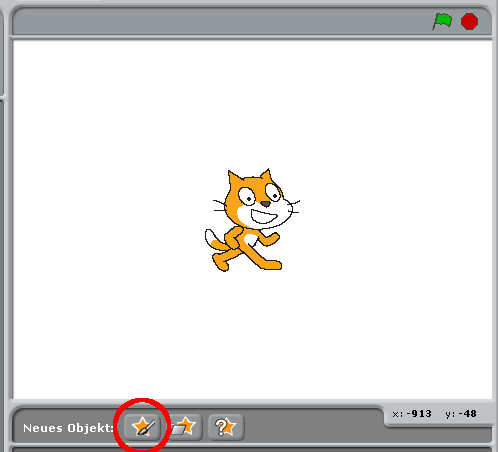
\includegraphics[width=0.6\textwidth]{images/aufgabe4_neues_objekt_malen.png}
\begin{enumerate}\addtocounter{enumi}{1}
\item Klicke auf das Quadrat, um das Rechteck-Tool auszuwählen.
\item Prüfe ob das ausgefüllte Quadrat unter den Werkzeugen selektiert ist.
\item Stelle sicher, dass die Farbe Schwarz ausgewählt ist
\item Zeichne nun durch gleichzeitiges Klicken und Ziehen mit der Maus ein Rechteck so wie es in folgendem Bild dargestellt ist.
\end{enumerate}
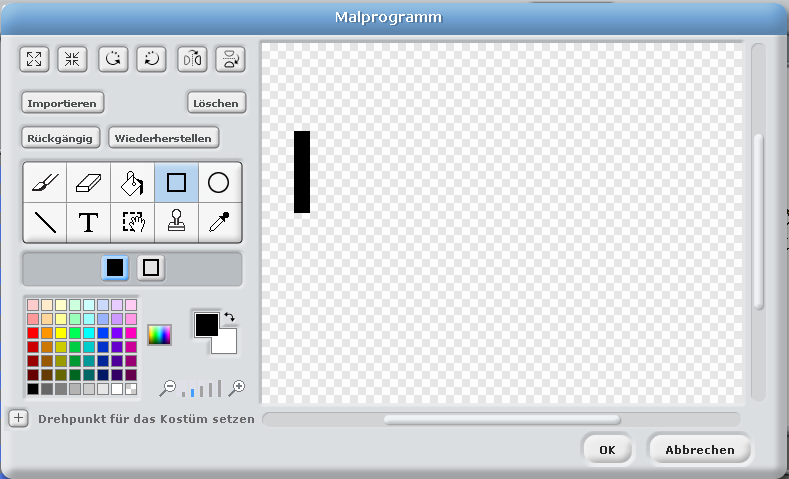
\includegraphics[width=0.6\textwidth]{images/aufgabe5_pong_sprite_spieler_malen.png}
\begin{enumerate}\addtocounter{enumi}{5}
\item Abschließend beende den Dialog durch betätigen der OK-Taste
\end{enumerate}
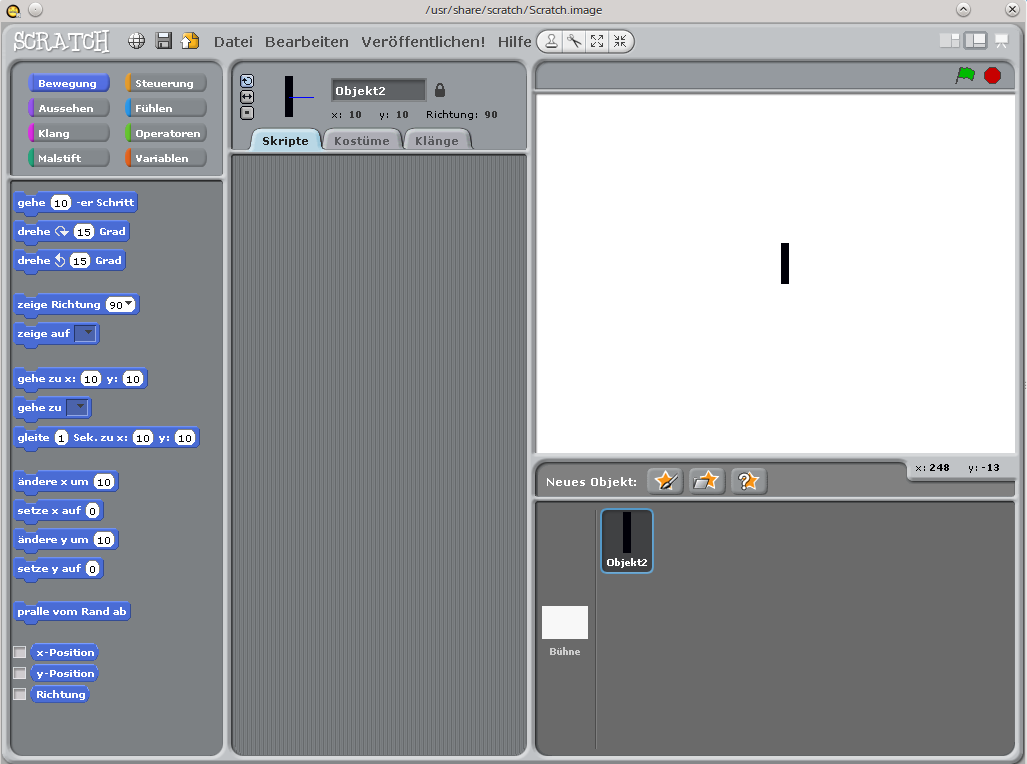
\includegraphics[width=0.6\textwidth]{images/aufgabe5_pong_sprite_spieler1_1.png}
\begin{enumerate}\addtocounter{enumi}{6}
\item Nun soll das neue Sprite noch den Namen \emph{Spieler1} erhalten
\item als letztes lösche das Objekt mit der Katze, sofern es noch vorhanden ist
\end{enumerate}
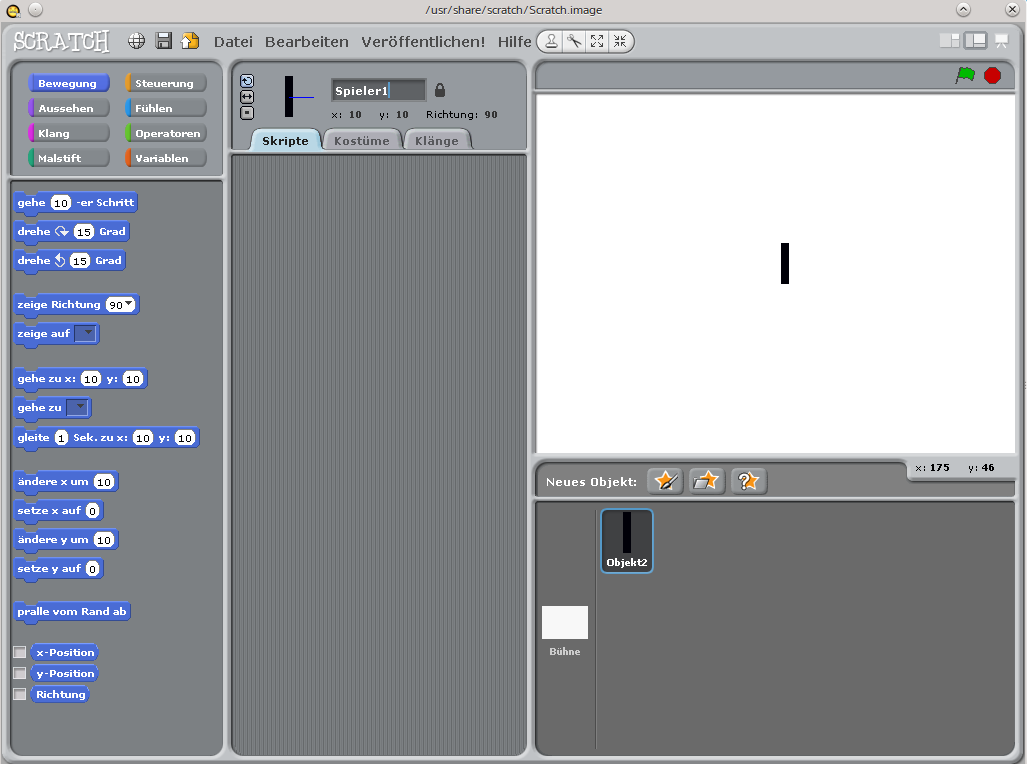
\includegraphics[width=0.6\textwidth]{images/aufgabe5_pong_sprite_spieler1_2.png}

\subsubsection{Programmiere das Verhalten des Spielers}

Nachdem nun der Spieler gemalt wurde muss sein Verhalten programmiert werden: Der Spieler soll durch betätigen der Taste \emph{w} nach oben und durch betätigen der Taste \emph{s} nach unten bewegt werden können.


\begin{enumerate}
\item Klicke auf den Sprite \emph{Spieler1}.
\item Für die Bewegung nach oben ziehe folgende Kacheln in dein Skript-Panel:
  \begin{enumerate}
  \item Aus dem Steuerungs-Panel die Kachel \textit{Wenn Taste Leertaste gedrückt} und \textit{wiederhole fortlaufend} und setze sie zusammen.
  \item Füge nun aus dem Steuerungs-Panel die Kachel \textit{warte bis} in die Schleife ein.
  \item Aus dem Fühlen-Panel die Kachel \textit{Taste ... gedrückt?}. Diese Kachel setzt du als Bedingung in die \textit{warte bis}-Kachel und wählst als Taste \emph{w} aus 
  \item Aus dem Bewegung-Panel suchst du die Kachel \textit{ändere y um ...} raus und fügst diese unter die Bedingung \textit{warte bis} ein. Setze den Wert in der Kachel auf \emph{10}    
  \end{enumerate}
\item Für die Bewegung nach unten dupliziere nun die eben angelegten Anweisungen und passe diese an:
  \begin{enumerate}
  \item passe die Kachel \textit{warte bis}-Kachel so an, dass auf die Taste \emph{s} gewartet wird
  \item ändere die Kachel \textit{ändere y um ...} auf \emph{-10}  
  \end{enumerate}
\item Damit der Spieler immer an der richtigen Stelle startet, ziehe folgende Kacheln in dein Skript-Panel:
  \begin{enumerate}
  \item Aus dem Steuerungs-Panel die Kachel \textit{Wenn Taste Leertaste gedrückt}
  \item Aus dem Aussehen-Panel die Kachel \textit{zeige dich} und füge sie an \textit{Wenn Taste Leertaste gedrückt}
  \item Aus dem Bewegung-Panel die Kachel \textit{gehe zu x: ... y: ...}, fügst diese an die Kachel \textit{zeige dich} und trägst für \emph{x} \emph{-200} und für \emph{y} \emph{0} ein.
  \end{enumerate}
\end{enumerate}

Damit ist der erste Spieler fertig. Dein Programm sollte nun so aussehen:

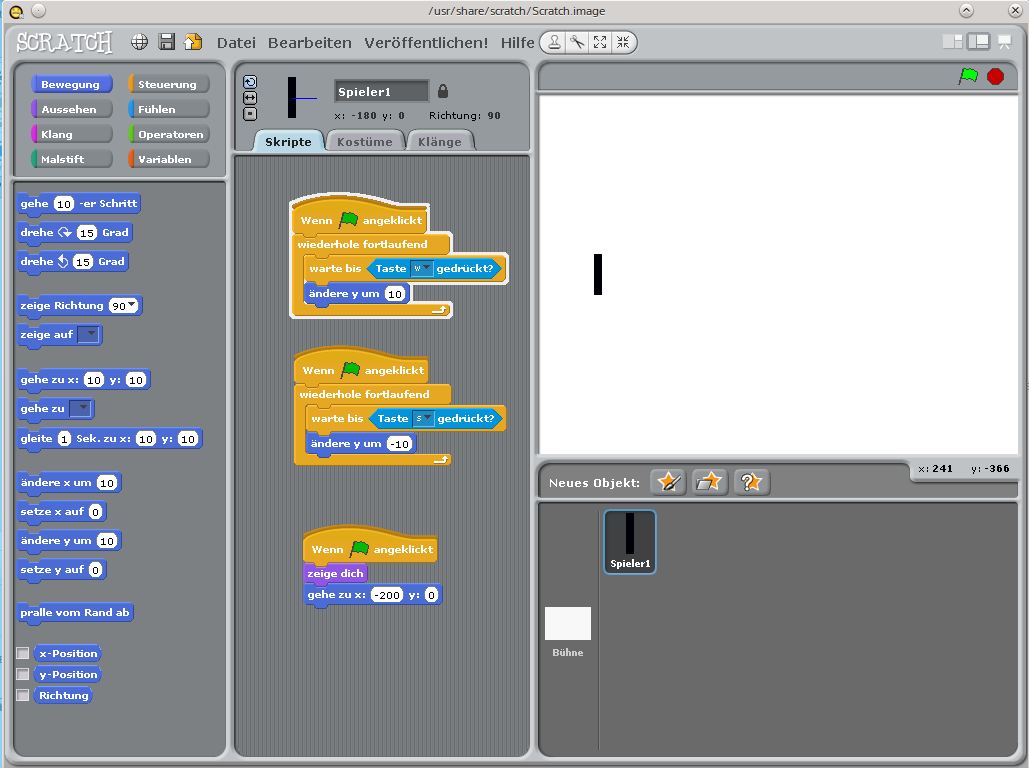
\includegraphics[width=0.6\textwidth]{images/aufgabe5_pong_sprite_spieler1_3.png}

Probiere ob du deinen Spieler mit den Tasten \emph{w} und \emph{s} steuern kannst.

\subsubsection{nun der zweite Spieler}

Den zweiten Spieler können wir durch kopieren des ersten erstellen. Anschließend müssen wir nur noch die Position auf dem Spielfeld und die Tasten für die Bewegung anpassen.

\begin{enumerate}
\item Wähle den Sprite \emph{Spieler1} und dupliziere ihn über den Menüeintrag im Kontextmenü (Das Menü erscheint, wenn du die rechte Maustaste auf dem Sprite betätigst)
\item Selektiere nun das neu erstellt Sprite und ändere seinen Namen auf \emph{Spieler2}
\item Ändere nun in der Kachel \textit{Taste w gedrückt?} die Taste auf \emph{o}
\item In der Kachel \textit{Taste s gedrückt?} änderst du die Taste auf \emph{l}
\item Abschließend ändere die \emph{x}-Position in der Kachel \textit{gehe zu x: -200 y: 0} auf \emph{200}
\end{enumerate}

Der zweite Spieler sollte nun so aussehen:

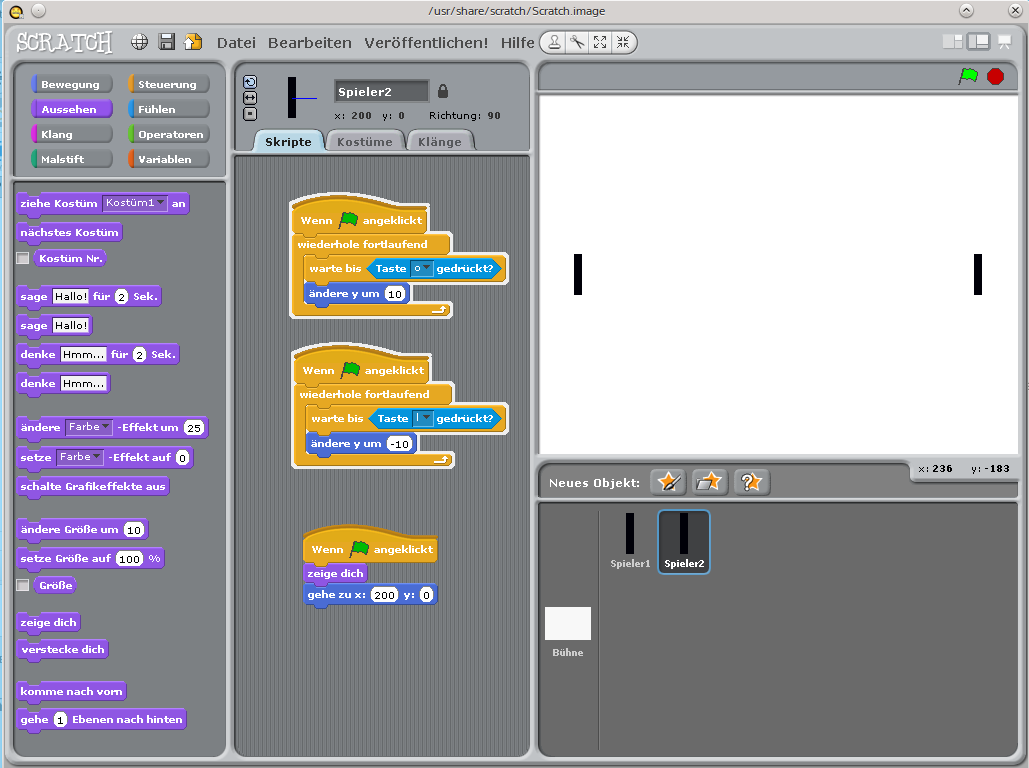
\includegraphics[width=0.6\textwidth]{images/aufgabe5_pong_sprite_spieler2.png}

Probiere aus, ob du beide Spieler mit den Tasten \emph{w,s} und \emph{o,l} bedienen kannst.

\subsection{Der Ball kommt ins Spiel}
Nun muss das Verhalten des Balls programmiert werden: Der Ball soll vom Rand abprallen. Wenn ein Spieler den Ball trifft, soll der Ball zurückgeschlagen werden. Trifft der Ball hinter einem Spieler auf den Rand, erhält der andere Spieler einen Punkt.

\subsubsection{Male einen Ball}
Zunächst klicke auf das \textit{Neues Objekt malen}-Icon, um einen Sprite für den Ball zu erzeugen. 
Du malst einen Ball mit Hilfe des Werkzeugs \emph{Ellipse}:

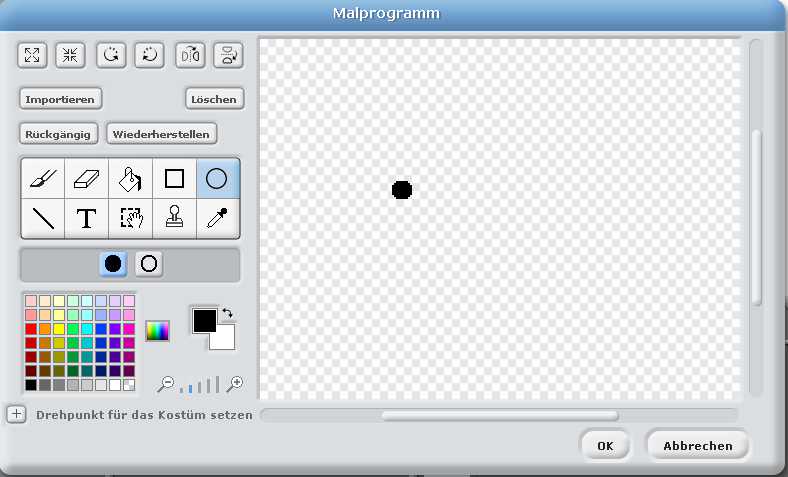
\includegraphics[width=0.6\textwidth]{images/aufgabe5_pong_sprite_ball_malen.png}


\subsubsection{Der Ball fliegt}
\begin{enumerate}
\item Selektiere nun das neu erstellt Sprite und ändere seinen Namen auf \emph{Ball}.
\item Füge nun die Kachel \textit{Wenn grüne Fahne angeklickt} dem Skript für den Ball zu.
\item Als nächsten initialisieren wir den Ball. 
Initialisieren bedeutet, beim Programmstart Dinge festzulegen, damit das Programm immer gleich abläuft. In unserem Fall bedeutet dies, beim Spielstart eine Ausgangssituation für den Ball festzulegen. So startet der Ball immer an der gleichen Position:
\begin{enumerate}
\item Füge die Kachel \textit{zeige dich} an die Kachel \textit{Wenn grüne Fahne angeklickt}
\item Als nächsten Befehl füge die Kachel \textit{gehe zu x: y:} an die Kachel \textit{zeige dich}. Setze den Wert für \emph{x} auf \emph{-200} und für \emph{y} auf \emph{0}
\item Am Spielbeginn soll der Ball in eine zufällige Richtung fliegen. Dies erreichst du indem, du die Kachel \textit{zeige Richtung} verwendest und als Wert die Kachel \textit{Zufallszahl von: bis:} einfügst. Trage für \emph{von} \emph{50} und für \emph{bis} \emph{130} ein.
\item Füge die fertige Kachel \textit{zeige Richtung} an die Kachel  \textit{gehe zu x: y:}  anfügst.
\end{enumerate}
\item Nach der Initialisierung kann nun der Ball zum Programmstart in eine zufällige Richtung zeigen, aber noch nicht bewegen. Das ist noch kein richtiges Spiel, daher sollen die nun folgenden Anweisungen immer wieder ausgeführt werden. Das erreichst du indem du die Kachel \textit{wiederhole fortlaufend} an die letzte Kachel deines Skripts anfügst 
\item nun kommen die Dinge, die der Ball immer wieder ausführen soll:
\begin{enumerate}
\item Als erstes soll der Ball von der Wand abprallen, wenn sie berührt. Dazu ziehst du die Kachel \textit{pralle von Rand ab} in die Schleife \textit{wiederhole fortlaufend}. 
\item Damit sich der Ball bewegt fügst du die Kachel \textit{gehe ... er Schritt} an die Kachel \textit{pralle von Rand ab}. Setze den Wert in der Kachel auf \emph{10}. Dieser Wert bestimmt wie schnell der Ball fliegt.  
\item Jetzt fehlt noch das Schlagen des Balls durch die Spieler. Durch den Schlag ändert der Ball zufällig seine Richtung:
\begin{enumerate}
\item Füge die Kachel \textit{falls} an die letzte Kachel in der Schleife ein.
\item Verwende als Bedingung für die Kachel \textit{wird ... berührt?} und wähle aus der Liste der Objekte dafür \emph{Spieler1}
\item Füge nun in die Kachel \textit{falls} die Kachel \textit{zeige Richtung ...}
\item Als Wert für die Richtung verwendest du die Kachel \textit{Zufallszahl von: bis:}.
\item Trage für \emph{von} \emph{50} und für \emph{bis} \emph{130} ein.
\end{enumerate}
\item Tue das Gleiche für den zweiten Spieler.
\item Für den zweiten Spieler muss der Wertebereich für die Zufallszahl \emph{von} \emph{-50}  \emph{bis} \emph{-130} gehen. 
\end{enumerate}
\end{enumerate}

So sollte dein Skript jetzt aussehen: 

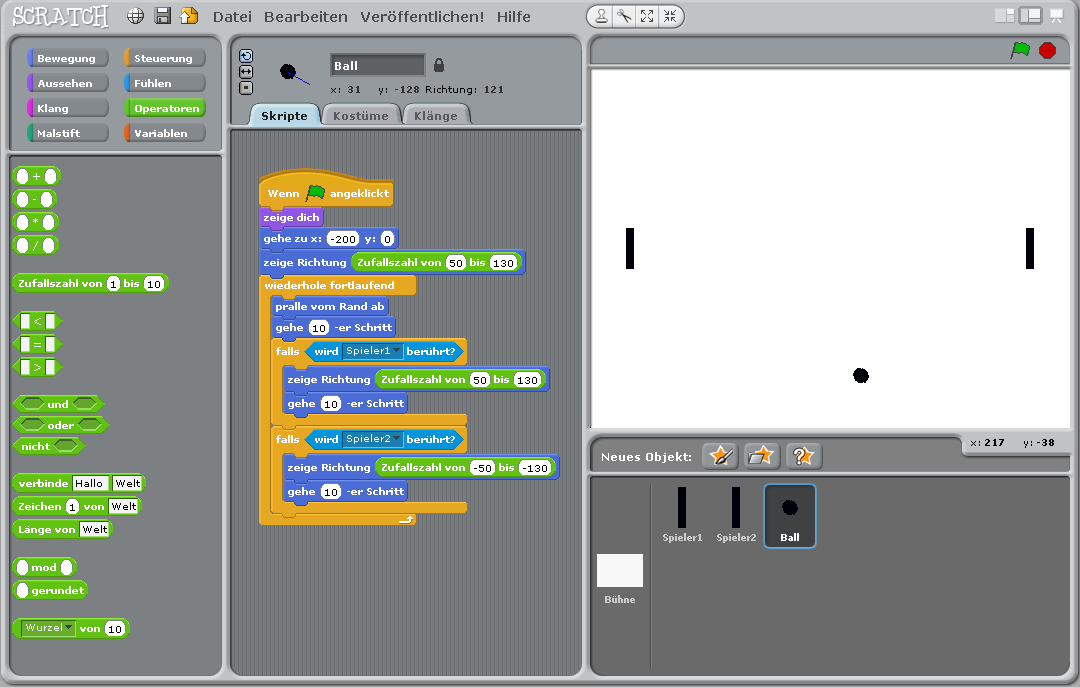
\includegraphics[width=0.6\textwidth]{images/aufgabe5_pong_sprite_ball_1.png}


\subsection{Der Hintergrund}

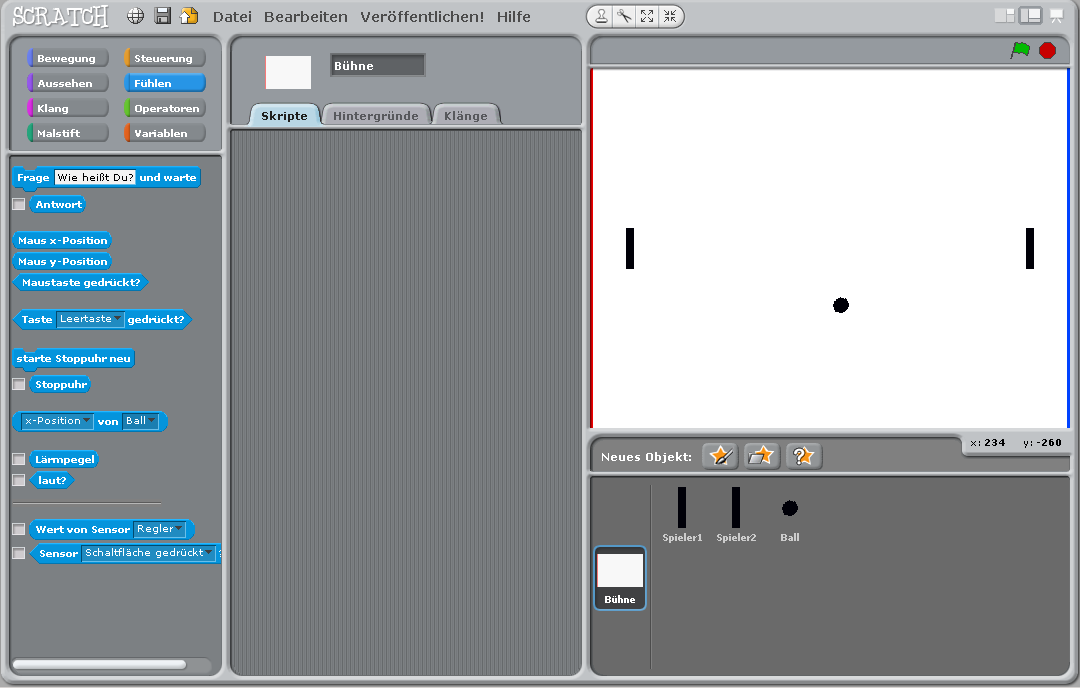
\includegraphics[width=0.6\textwidth]{images/aufgabe5_pong_hintergrund_1.png}
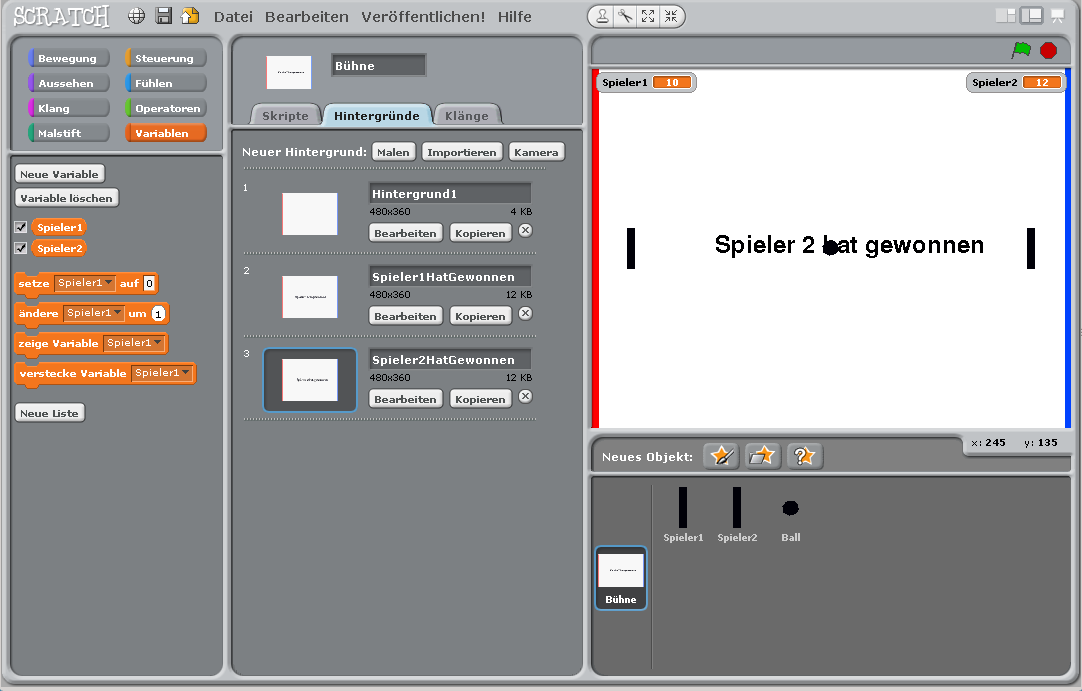
\includegraphics[width=0.6\textwidth]{images/aufgabe5_pong_hintergrund_2.png}
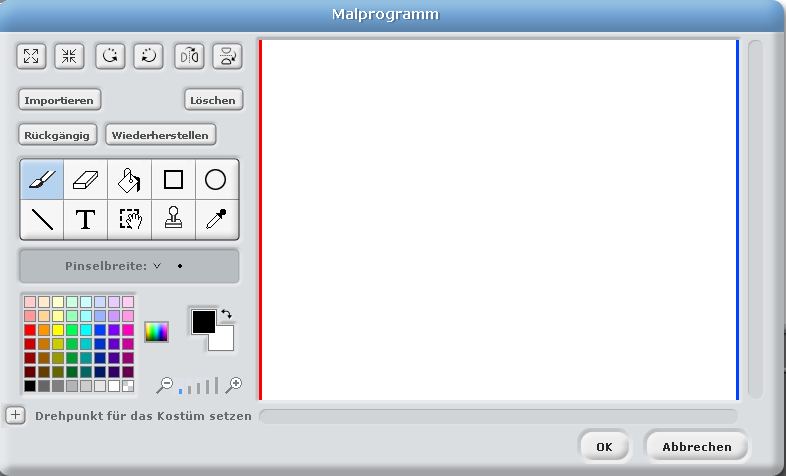
\includegraphics[width=0.6\textwidth]{images/aufgabe5_pong_hintergrund_malen.png}


\subsection{Wer hat gewonnen?}
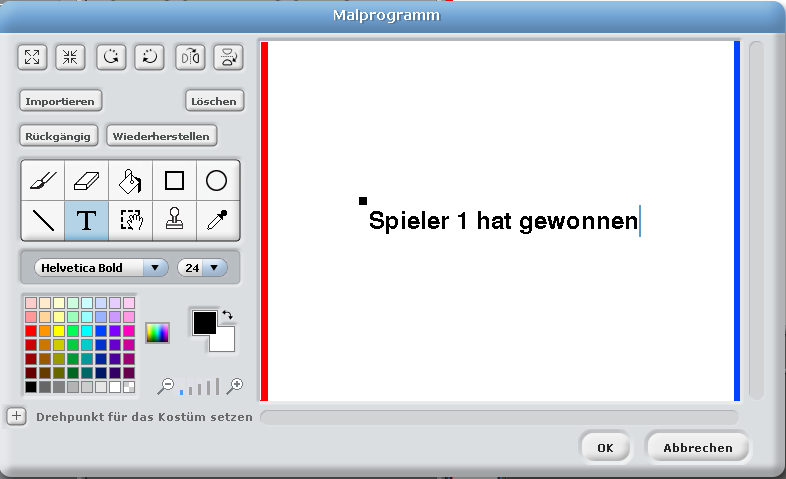
\includegraphics[width=0.6\textwidth]{images/aufgabe5_pong_hintergrund_gewonnen_malen.png}
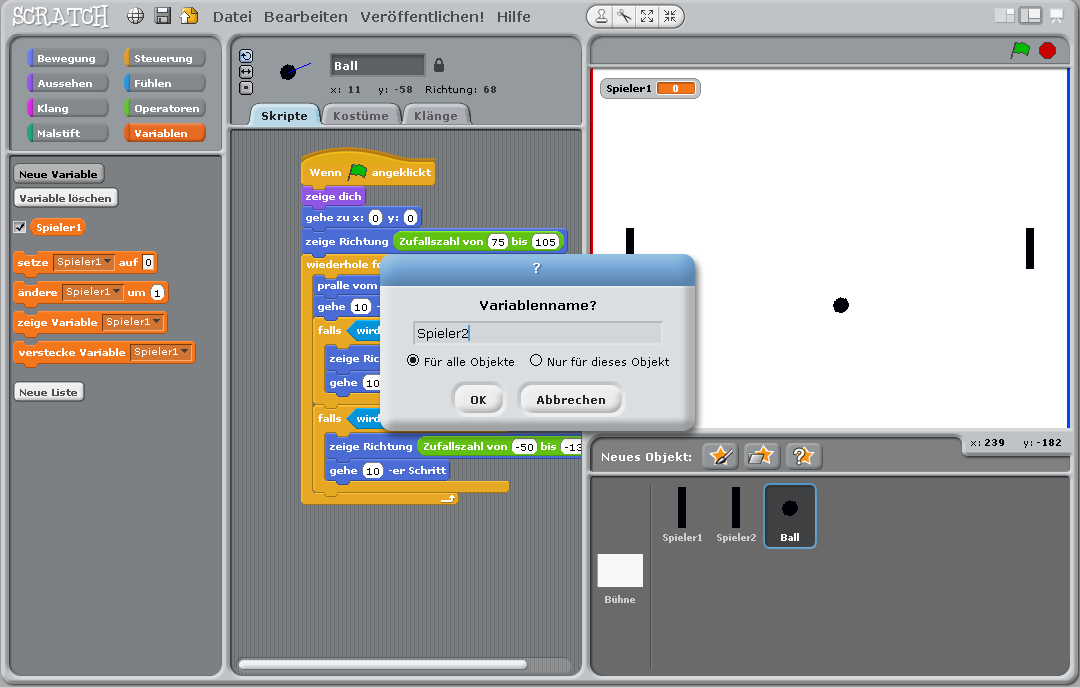
\includegraphics[width=0.6\textwidth]{images/aufgabe5_pong_spieler_variablen_1.png}

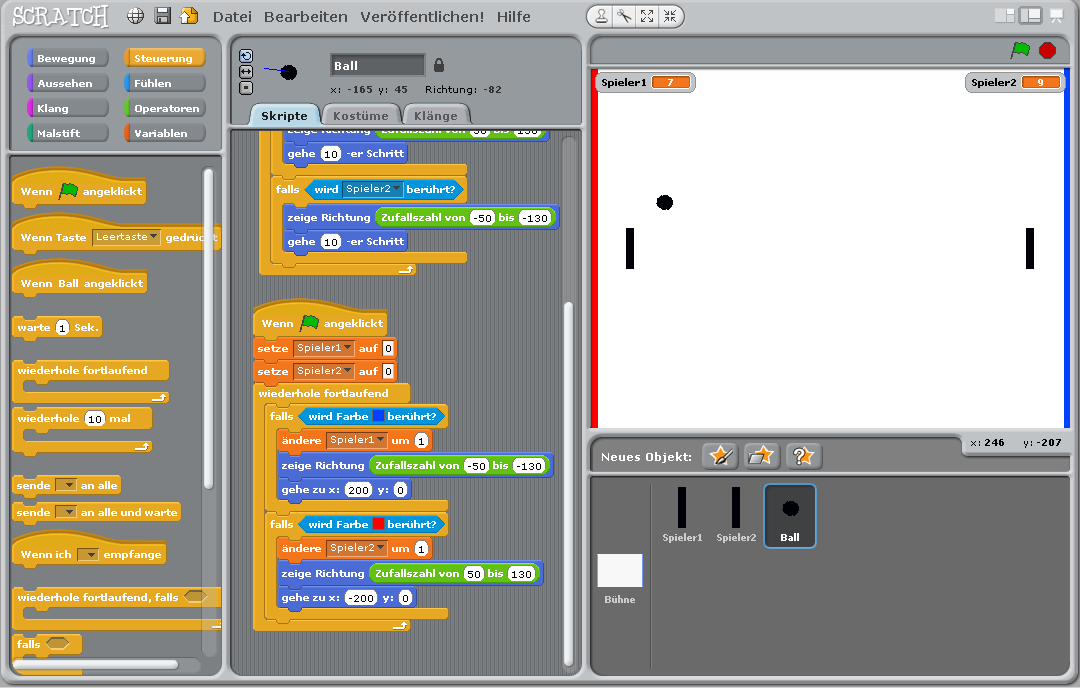
\includegraphics[width=0.6\textwidth]{images/aufgabe5_pong_spieler_variablen_2.png}
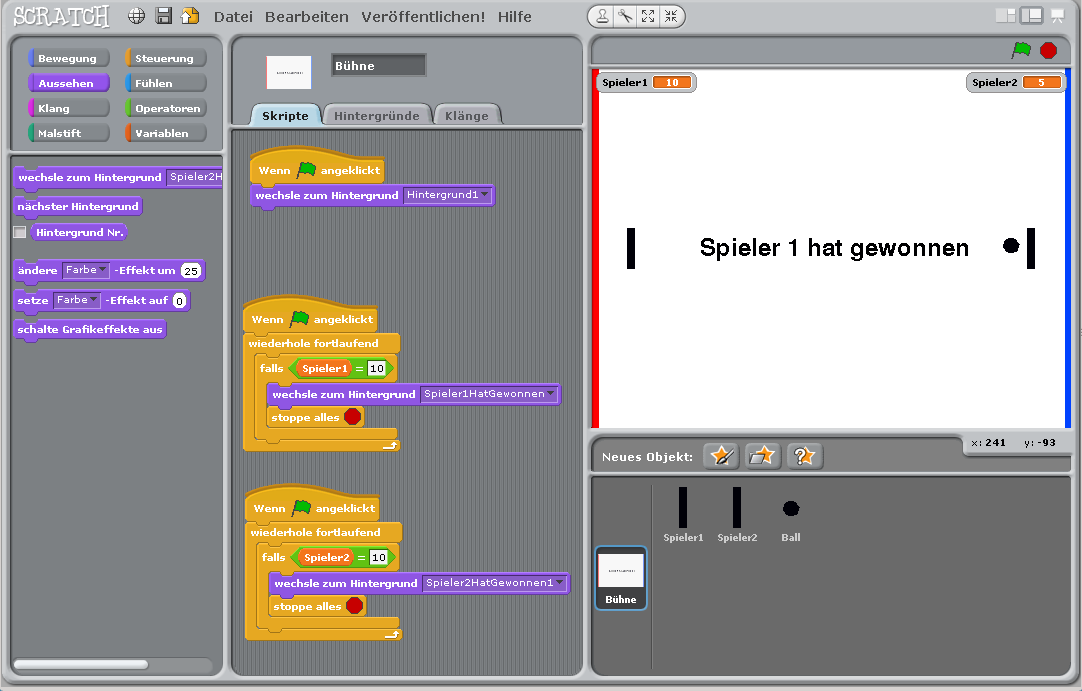
\includegraphics[width=0.6\textwidth]{images/aufgabe5_pong_spieler_variablen_3.png}

\subsection{Erweiterungen}
Das Pong-Spiel ist nun ersteinmal fertig, dennoch kannst du es erweitern:

\begin{enumerate}
\item Versuche das Programm so zu erweitern, dass der Ball schneller wird sobald ein Spieler den Ball getroffen hat. Du brauchst dafür eine weitere Variable, die die Geschwindigkeit des Balls enthält.
\item Die Auslinien sind durch die rote und blaue Linie im Hintergrund dargestellt. Gezählt wird, wenn der Ball die rote oder blaue Farbe berührt. Überlege wie du das Programm umbauen müsstest, wenn die Auslinien selbst Objekte sind. Diese Objekt sollen merken können sobald sie der Ball trifft und die Punkte entsprechend anpassen.
\item Nachdem die Auslinien Objekte geworden sind, kannst du aus dem Tennisspiel ein Fußballspiel machen. Hierzu brauchst du nur die Auslinien auf Torlänge zu kürzen. 
\end{enumerate}









\begin{itemize}
\item[1. ] Klicke auf das \textit{Neues Objekt malen}-Icon
\end{itemize}

\begin{itemize}
\item[2. ] Benutze das Zoom-Tool um komplett herauszuzoomen. Klicke auf die Minus-Lupe.
\end{itemize}

\begin{itemize}
\item[3. ] Klicke auf den Pinsel um diesen auszuwählen, wähle einen dickeren Pinsel und die Farbe grau.
\end{itemize}

\begin{itemize}
\item[4. ] Benutze den Pinsel um eine Rennbahn zu malen.
\end{itemize}

\begin{itemize}
\item[5. ] Da das jetzt einer Rennbahn noch nicht so ähnlich sieht füllen wir die Rennfläche mit der Farbe \emph{hellgrün} und den Berg in der Mitte mit der Farbe \emph{braun} und alles andere Hellblau. Du kannst die Flächen mit dem Pinsel anmalen, leichter ist es jedoch mit dem \emph{Farbeimer}. Dazu einfach den Farbeimer und die Farbe auswählen und dann auf die gewünschte Fläche klicken.
\end{itemize}

\begin{itemize}
\item[6. ] Zum Schluss fügen wir noch ein weiteren Sprite hinzu und zwar eine \emph{Start/Ziel-Linie} in der Farbe \emph{rot}, diese erstellen und auf die gewünschte Position schieben.
\end{itemize}

\begin{itemize}
\item[7.] Ändere den Namen des Sprites zu \textit{Rennbahn} und den Namen des Sprites für die Start/Ziel-Linie zu \textit{Start/Ziel}.
\end{itemize}

\subsection{Katze einfügen}

\begin{itemize}
\item[1.] Füge den Sprite \emph{Katze} aus einer Datei hinzu.
\end{itemize}

\begin{itemize}
\item[2. ] Ändere den Namen des Sprites zu Katze.
\end{itemize}
\begin{itemize}
\item[3.] Benutze das Verkleinerungs-Tool, um die Größe deiner Katze soweit zu verkleinern, dass sie zur Größe der Bahn passt und ohne anzustoßen auf der Bahn laufen kann.
\end{itemize}


\subsection{Erzeuge das Script für die Steuerung der Katze}

\begin{itemize}
\item[1. ] Klicke auf den Sprite Katze.
\item[2. ] Ziehe folgende Kacheln in dein Skript-Panel:
  \begin{itemize}
  \item[1. ] Aus dem Steuerungs-Panel die Kachel \textit{Wenn Taste Leertaste gedrückt} und \textit{falls...sonst} und setze beide zusammen.
  \item[2. ] Aus dem Fühlen-Panel die Kachel \textit{wird Farbe berührt}. Diese Kachel setzt du als Bedingung in die \textit{falls...sonst}-Kachel
  \item[3. ] Aus dem Aussehen-Panel suchst du die Kachel \textit{sage Hallo! für 2 Sek.} raus und fügst diese in den Bereich \textit{falls}, der \textit{falls...sonst}-Kachel ein.
  \item[4. ] Im Bewegungs-Panel findest du nun die vier letzten Kacheln für die Steuerung der Katze: \textit{zeige in Richtung 90} und \textit{gehe zu} fügst du in den \textit{falls}-Bereich, gleich nach der Kachel \textit{sage Hallo! für 2 Sek.} ein. In den \textit{sonst}-Bereich ziehst du die beiden Kacheln \textit{zeige in Richtung 90} und \textit{gehe 10-er Schritt}.
  \end{itemize}
\end{itemize}

\begin{itemize}
\item[3. ] Bei der Kachel \textit{Wenn Taste Leertaste gedrückt} klickst du auf den Text \textit{Leertaste} und w{\"a}hlst aus der Liste \textit{Pfeil nach oben}.
\item[4. ] Bei der Kachel \textit{wird Farbe berührt} auf die Farbe klicken und dann auf den grauen Rand unserer Rennbahn.
\item[5. ] Bei der Kachel \textit{sage Hallo! für 2 Sek.} auf den Text \textit{Hallo!} klicken und diesen zu \textit{Au!} ändern.
\item[6. ] Bei der Kachel \textit{zeige in Richtung 90} im \textit{falls}-Bereich auf die Zahl \textit{90} klicken und aus der Liste \textit{(-90) links} auswählen.
\item[7. ] Bei der Kachel \textit{gehe zu} auf den kleinen Pfeil klicken und unseren Sprite \textit{Start/Ziel} aus der Liste auswählen.
\item[7. ] Bei der Kachel \textit{zeige in Richtung 90} im \textit{sonst}-Bereich auf die Zahl \textit{90} klicken und aus der Liste \textit{(0) oben} auswählen.
\item[8. ] Bei der letzten Kachel \textit{gehe 10-er Schritt} soll die Zahl \textit{10} durch eine \textit{2} ersetzt werden.
\end{itemize}


\begin{itemize}
\item[9. ] Das Ganze jeweils für die drei restlichen Richtungen \textit{rechts}, \textit{unten} und \textit{links} wiederholen und dabei nicht vergessen bei der Kachel \textit{zeige in Richtung 90} jeweils die gewünschte Richtung auswählen und die richtige Taste zu ändern.
\end{itemize}


\begin{itemize}
\item[10. ] Um die Katze beim Start des Spiels zur Startlinie zu bringen, füge die Kacheln \textit{Wenn Fahne angeklickt} aus dem Steuerungs-Panel, aus dem Bewegungs-Panel \textit{zeige Richtung 90} und \textit{gehe zu} ein und setze diese zusammen.
\item[11. ] Bei der Kachel \textit{zeige in Richtung 90} im \textit{sonst}-Bereich auf die Zahl \textit{90} klicken und aus der Liste \textit{(-90) links} auswählen.
\item[12. ] Bei der Kachel \textit{gehe zu} auf den Pfeil klicken und aus dem Menü und \textit{Start/Ziel} auswählen.
\end{itemize}


\subsection{Zusatzaufgabe: Erweitere das Spiel damit zwei Spieler spielen können}
Du kannst einen weiteren Sprite hinzufügen und dir weitere vier Tasten auf der Tastatur aussuchen um diesen auch eine Steuerung zu geben. Hier die kurze Beschreibung wie man das machen könnte:
\begin{itemize}
\item[1. ] Die vier Tasten für die Steuerung überlegen z.B.
  \begin{itemize}
  \item w = oben
  \item d = rechts
  \item s = unten
  \item a = links
\end{itemize}
\item[2. ] Kopiere die Katze und passe die Skripte an, sodass die von dir ausgewählten Tasten zur Steuerung der Katze benutzt werden]
  \item[3. ] Ändere das Aussehen einer Katze um es leichter zu machen sie zu Unterscheiden (wir haben ihr ein paar Punkte gegeben).
\end{itemize}

